\section{$H$-Methode}
\begin{frame}
  \frametitle{Vergleich von Methoden}
  \begin{figure}
	  \caption{Quelle: \emph{A. T. Endo and A. Simao, "Experimental Comparison of Test Case Generation Methods for Finite State Machines," 2012 IEEE Fifth International Conference on Software Testing, Verification and Validation, Montreal, QC, 2012, pp. 549-558.} }
	  \centering
	  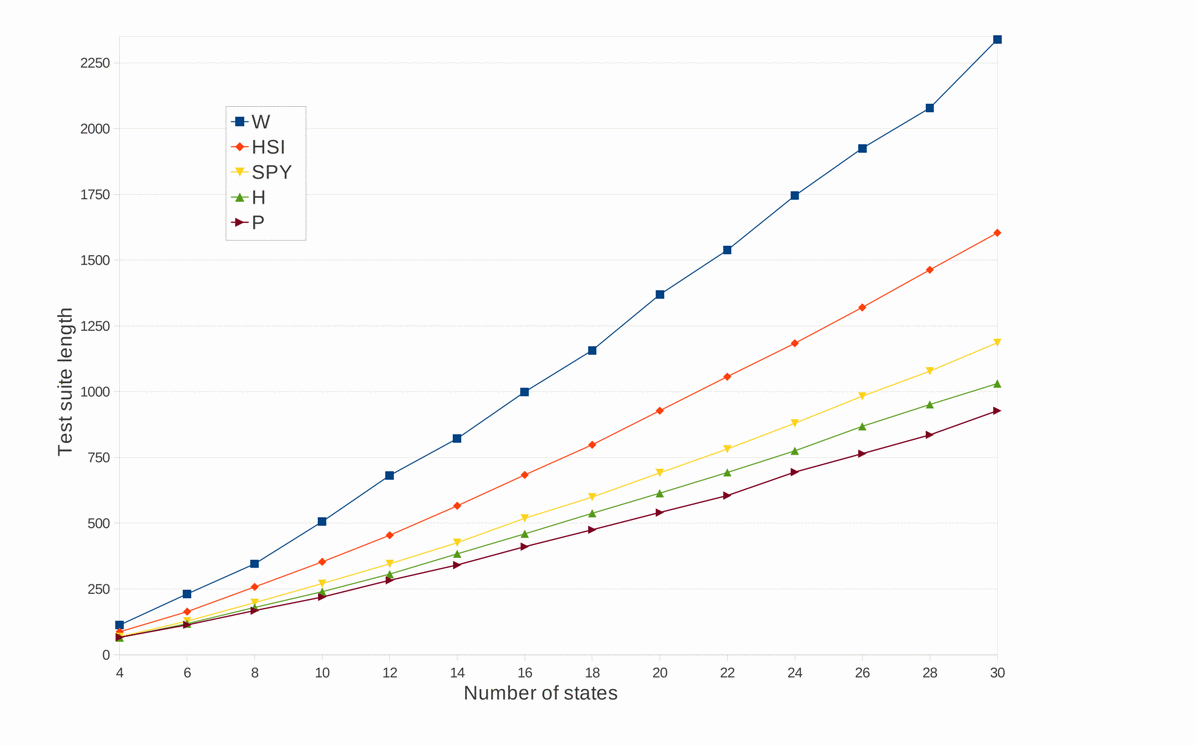
\includegraphics[width=0.85\textwidth]{images/methodComparison}
	\end{figure}

\end{frame}

\begin{frame}
  \frametitle{$H$-Methode}
  DFSM sei vollständig und minimal
  \begin{itemize}
    \item $A=V\times V$
  	\item $B=V\times (V.\bigcup\limits_{i=1}^{m-n+1}.\Sigma_I^i)$
  	\item $C=\{(\alpha,\beta)|\alpha,\beta\in V.\bigcup\limits_{i=1}^{m-n+1}.\Sigma_I^i, \alpha \in \text{Pref}(\beta)\}$
  \end{itemize}
  Für alle Paare $(\alpha, \beta) \in A\cup B \cup C$, falls $\delta(q_0,\alpha) \not \sim \delta(q_0,\beta)$, dann enthält die Test Suite $\alpha.\omega,\beta.\omega$. $\omega$ ist die \emph{distinguishing trace} für $\delta(\alpha)$ und $\delta(\beta)$.
\end{frame}

\begin{frame}
\frametitle{$H$-Methode - Beispiel}
\begin{columns}[T] % align columns

\begin{column}{.4\textwidth}
\textbf{Liste von Paaren $(\alpha,\beta)$}\\
  \begin{itemize}
	\item<1>$V.\bigcup\limits_{i=1}^{m-n+1}.\Sigma_I^i$
	\item<2-3>\only<1-2>{$(aa,b)$}\only<3->{$(aa,b) \rightarrow a$}
    \item<4-5>\only<1-4>{$(aa,\epsilon)$}\only<5->{$(aa,\epsilon) \rightarrow b$}
    \item<6-7>\only<1-6>{$(ba,a)$}\only<7->{$(ba,a) \rightarrow a$}
    \item<8-9>\only<1-8>{$(ba,\epsilon)$}\only<9->{$(ba,\epsilon) \rightarrow a$}
    \item<10-11>\only<1-10>{$(ab,a)$}\only<11->{$(ab,a) \rightarrow a$}
    \item<12-13>\only<1-12>{$(bb,a)$}\only<13->{$(bb,a) \rightarrow b$}
  \end{itemize}
\end{column}%

\begin{column}{.70\textwidth}
\centering
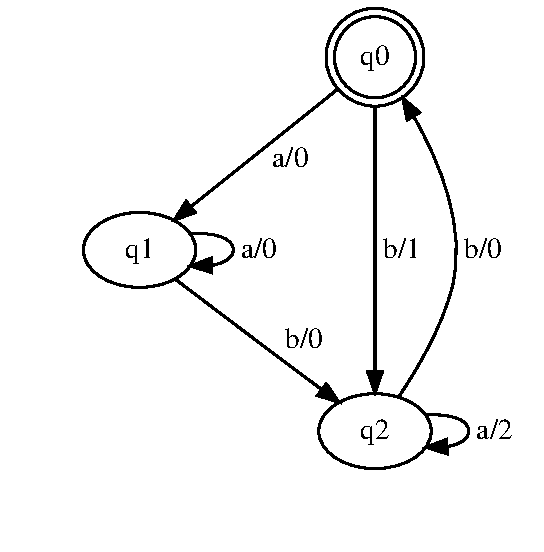
\includegraphics[width=0.5\textwidth]{images/fsm-example01_orig}%
\only<1-2>{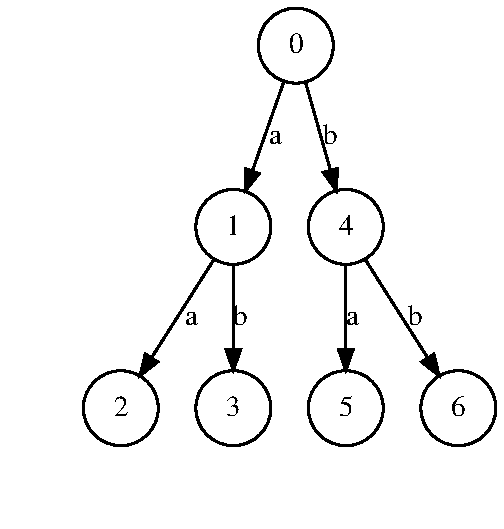
\includegraphics[width=0.5\textwidth]{images/HTree01}}%
\only<3>{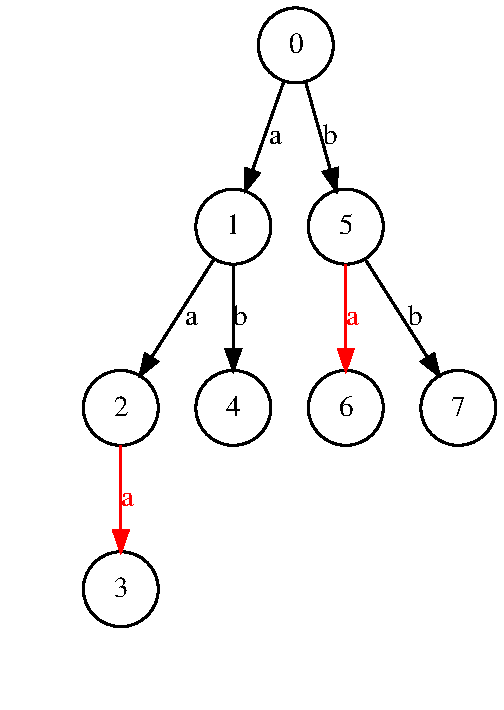
\includegraphics[width=0.5\textwidth]{images/HTree02_c}}%
\only<4>{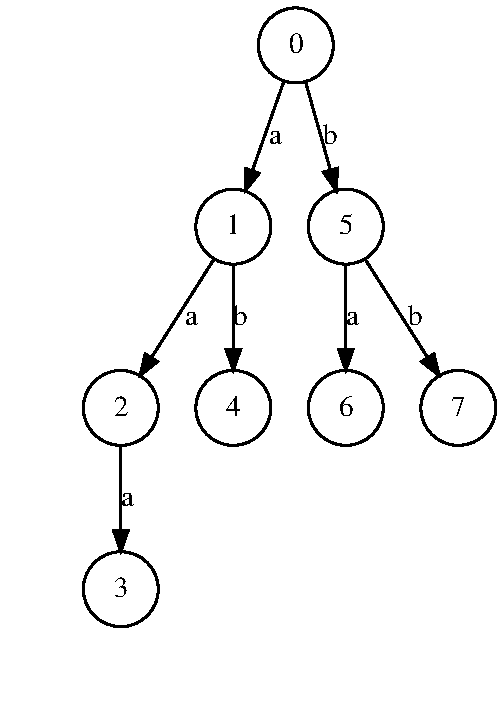
\includegraphics[width=0.5\textwidth]{images/HTree02}}%
\only<5>{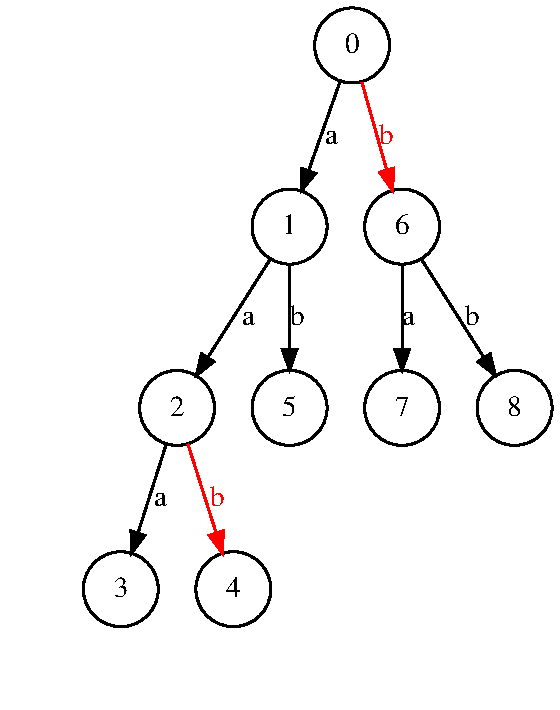
\includegraphics[height=0.6\textheight]{images/HTree03_c}}%
\only<6>{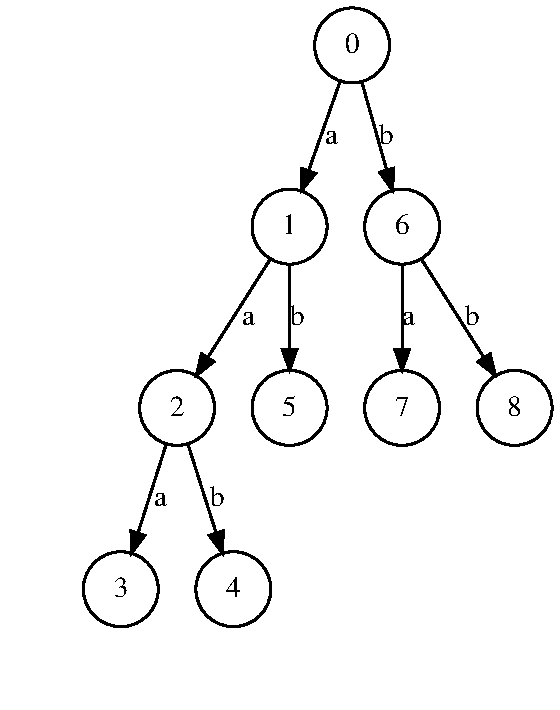
\includegraphics[height=0.6\textheight]{images/HTree03}}%
\only<7>{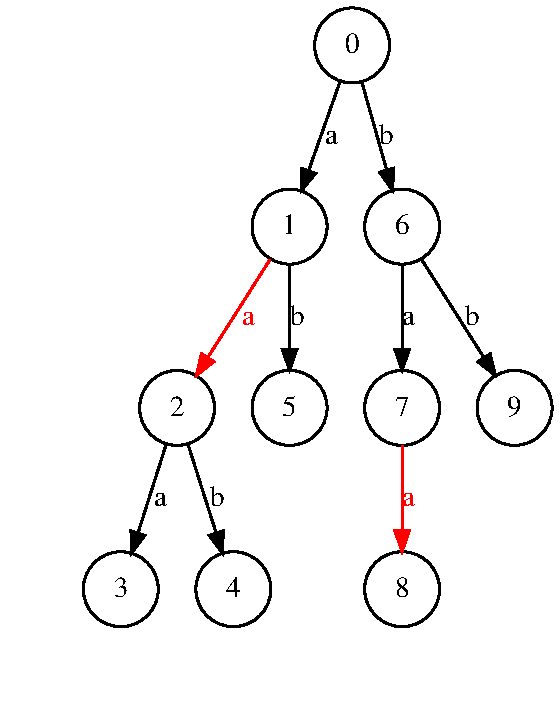
\includegraphics[height=0.6\textheight]{images/HTree04_c}}%
\only<8>{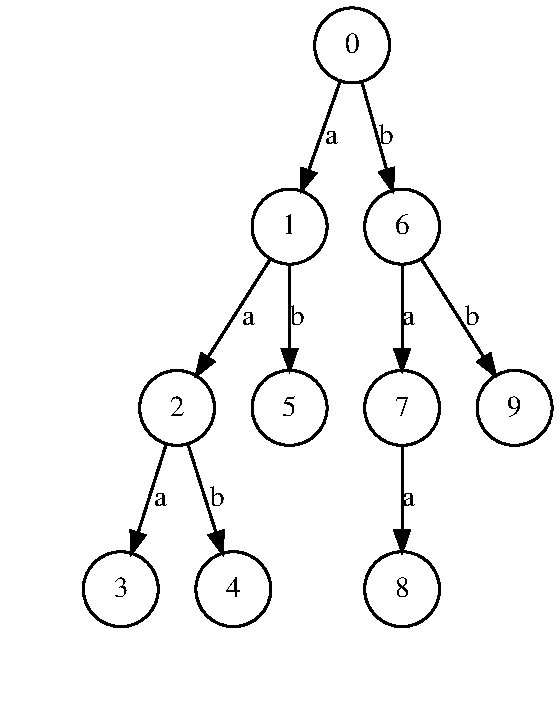
\includegraphics[height=0.6\textheight]{images/HTree04}}%
\only<9>{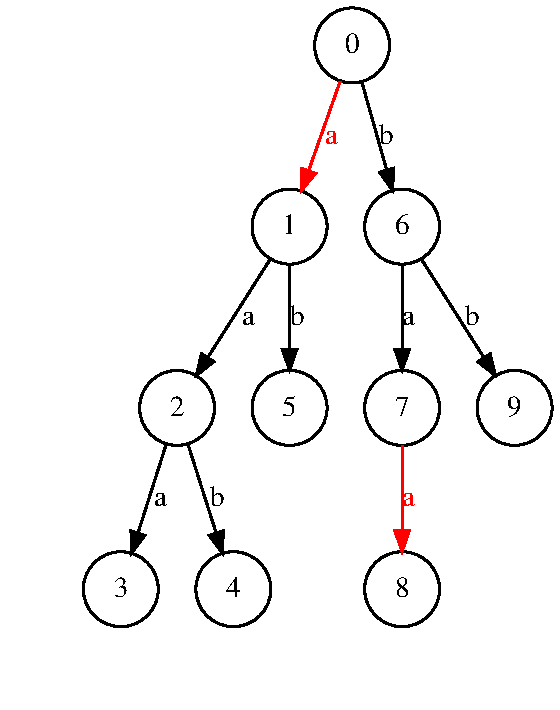
\includegraphics[height=0.6\textheight]{images/HTree05_c}}%
\only<10>{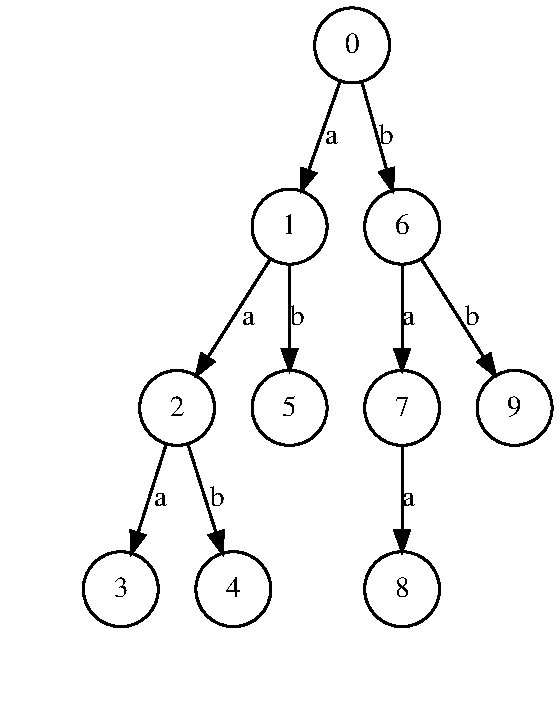
\includegraphics[height=0.6\textheight]{images/HTree05}}%
\only<11>{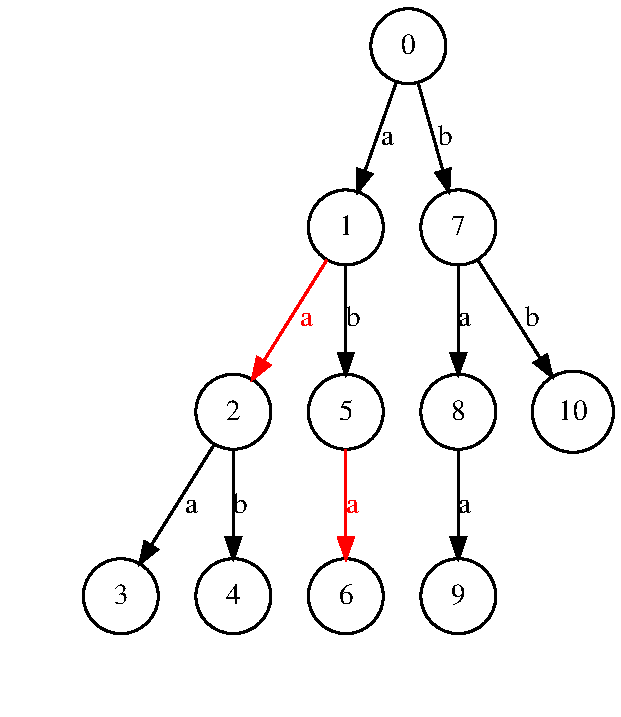
\includegraphics[height=0.6\textheight]{images/HTree06_c}}%
\only<12>{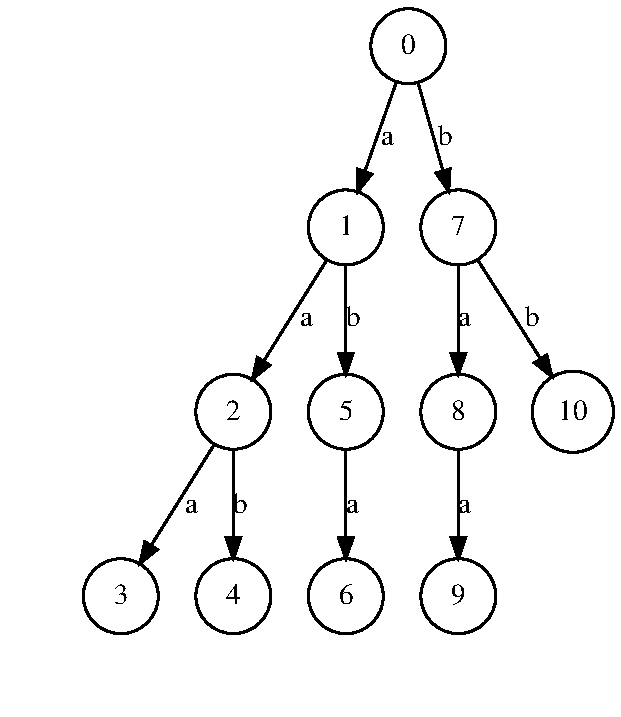
\includegraphics[height=0.6\textheight]{images/HTree06}}%
\only<13>{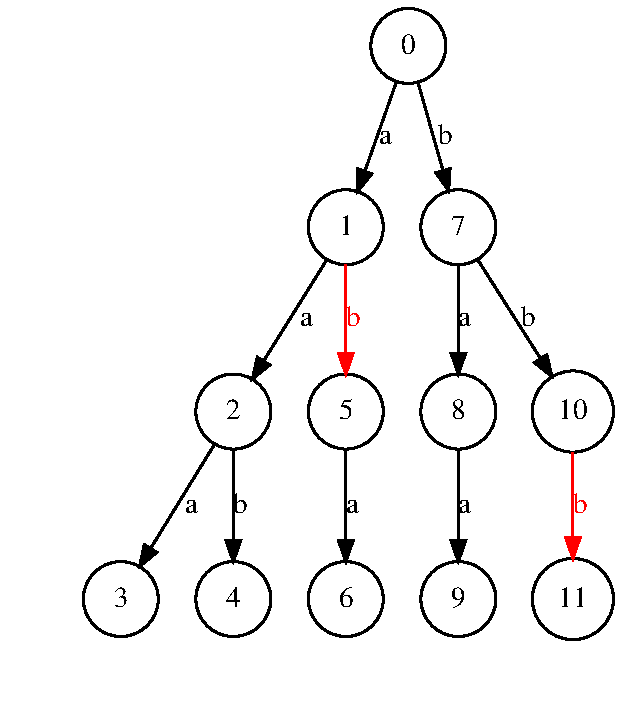
\includegraphics[height=0.6\textheight]{images/HTree07_c}}%
\only<14>{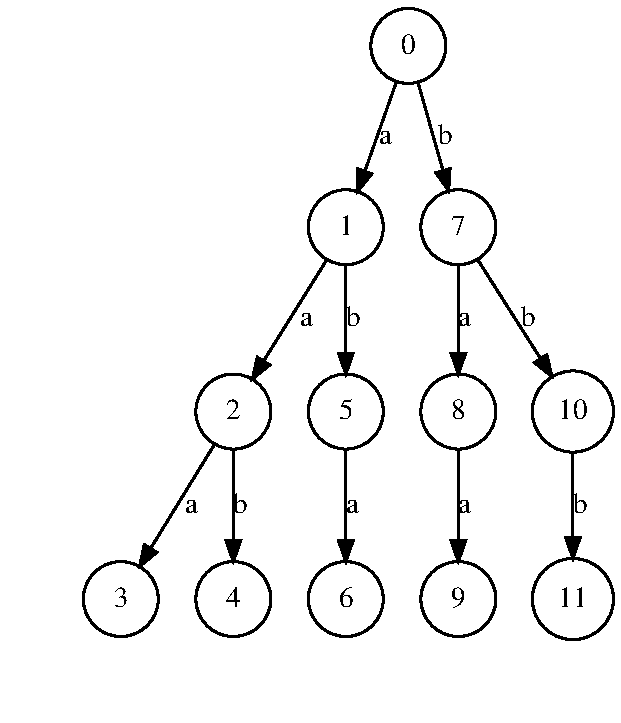
\includegraphics[height=0.6\textheight]{images/HTree07}}%
\end{column}%

\end{columns}
\end{frame}

\begin{frame}
\frametitle{$H$-Methode - Vergleich}
\begin{columns}[T] % align columns

\begin{column}{.7\textwidth}
\begin{itemize}[<+->]
    \item $\W$-Methode: 8 Testfälle, 24 Testschritte
    \item $\W_p$-Methode: 7 Testfälle, 21 Testschritte
    \item $H$-Methode: 5 Testfälle, 15 Testschritte
\end{itemize}
\end{column}%

\begin{column}{.50\textwidth}
\centering
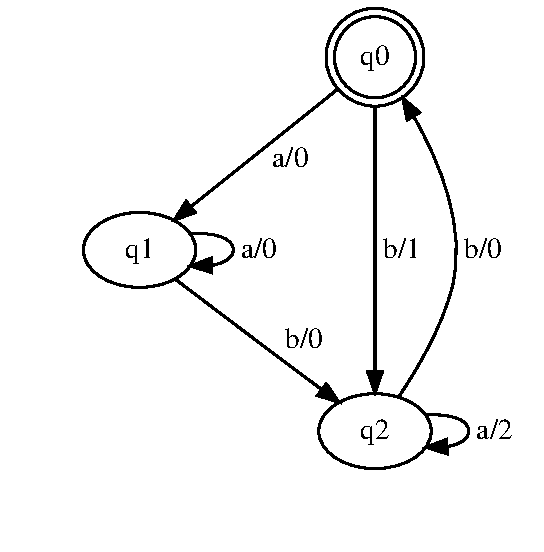
\includegraphics[width=\textwidth]{images/fsm-example01_orig}%
\end{column}%

\end{columns}
\end{frame}

\begin{frame}
\frametitle{$H$-Methode - Optimierung}
Wahl von $\omega$ vom aktuellen Testbaum abhängig machen.

\begin{itemize}
      \item<2-> Ideal: Für $(\alpha, \beta$) finde $\omega$, sodass $\alpha.\omega$ und $\beta.\omega$ im Testbaum
      \item<3-> Sonst: Erweitere bestehenden Test
      \item<4-> Wenn nicht anders möglich: Neuer Testfall 
    \end{itemize}
\end{frame}

\begin{frame}
  \frametitle{$H$-Methode - Optimierung}

  \begin{columns}[T] % align columns
    \begin{column}{.3\textwidth}
	    \begin{itemize}
		  \item Betrachte $(c.a,d)$
		  \item mögliches $\omega: e$
	    \end{itemize}
    \end{column}%

    \begin{column}{.70\textwidth}
        \only<1->{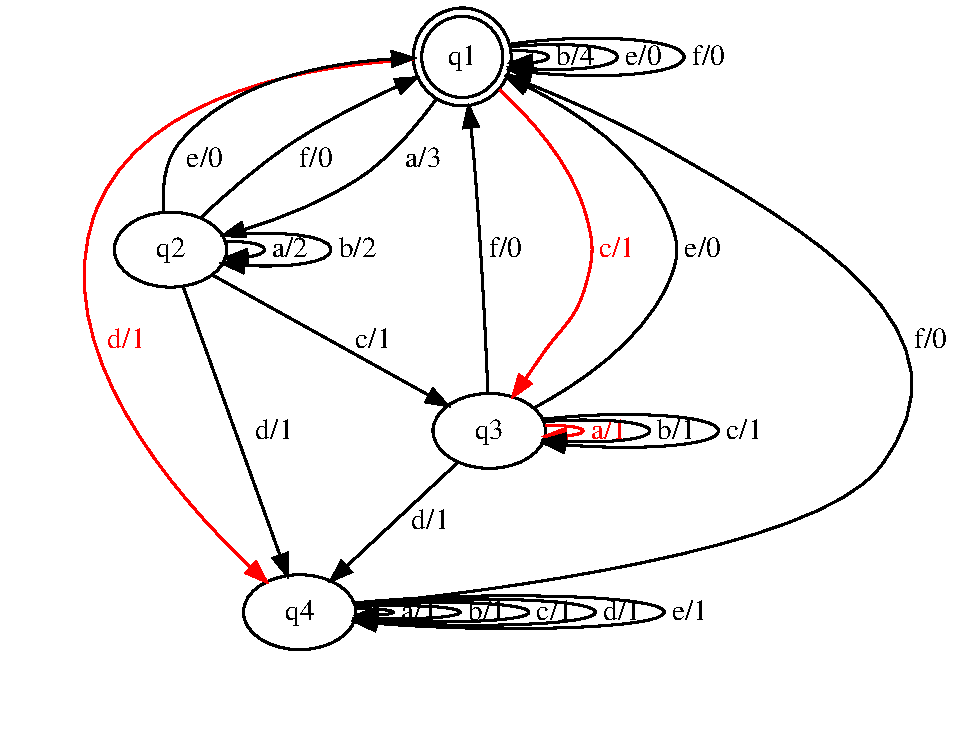
\includegraphics[width=\textwidth]{images/FSM_opt}}
    \end{column}%
  \end{columns}
\end{frame}


\begin{frame}
  \frametitle{$H$-Methode - Optimierung}
  \begin{columns}[T] % align columns

\begin{column}{.4\textwidth}
  \begin{itemize}
	\item<2->Wahl $e$ für $\omega$ würde neuen Test erzeugen
	\item<3->Versuche bestehenden Test zu erweitern
	\item<4->$a.e$ statt $e$
  \end{itemize}
\end{column}%

\begin{column}{.70\textwidth}
Zu diesem Zeitpunkt sieht der Testbaum so aus:
\only<1>{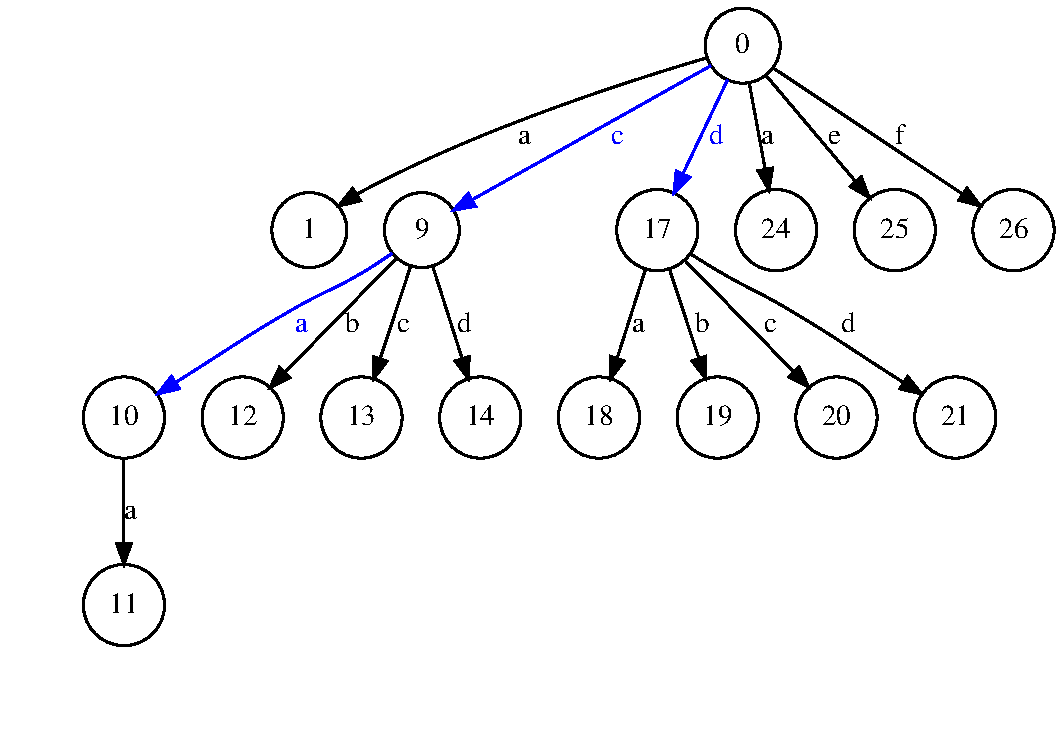
\includegraphics[height=0.6\textheight]{images/HTree_opt}}
\only<2-3>{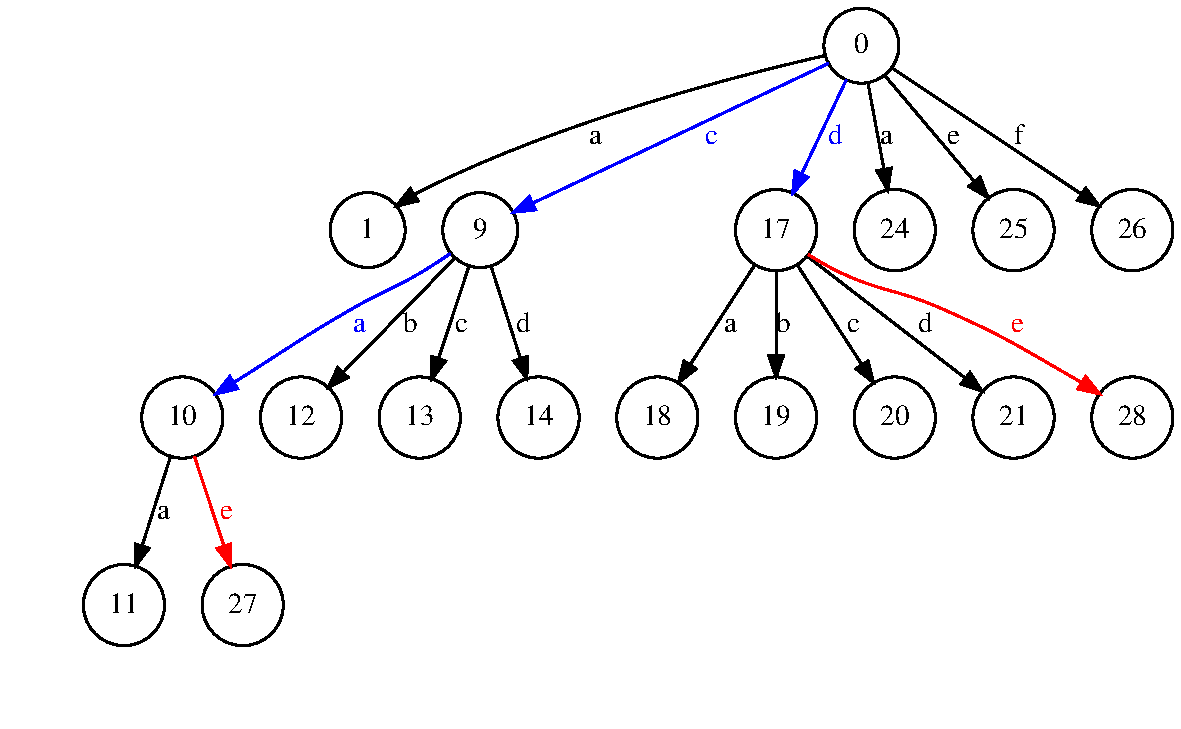
\includegraphics[height=0.6\textheight]{images/HTree_opt2}}
\only<4->{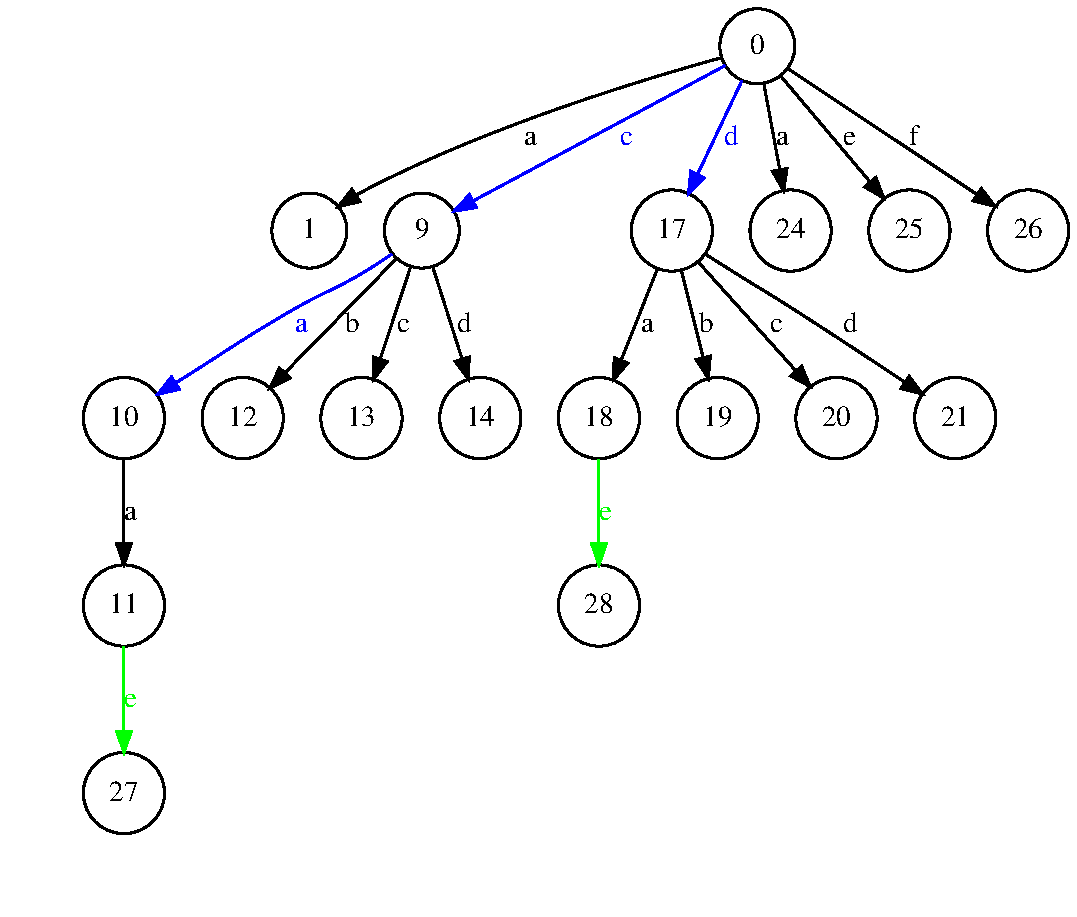
\includegraphics[height=0.7\textheight]{images/HTree_opt3}}
\end{column}%

\end{columns}

\end{frame}